%%%%%%%%%%%%%%%%%%%%%%%%%%%%%%%%%%%%%%%%%%%%%%%%%%%%%%%%%%%%%%%%%%%%%%%%
%%% Anonymous AAMAS 2027 submission draft.
%%% Official template downloaded 2026-09-11 from the AAMAS 2027 site.
%%%%%%%%%%%%%%%%%%%%%%%%%%%%%%%%%%%%%%%%%%%%%%%%%%%%%%%%%%%%%%%%%%%%%%%%

\documentclass[sigconf,anonymous]{aamas}

\usepackage{booktabs}
\usepackage{graphicx}
\usepackage{amsmath}

%%% AAMAS-2027 copyright block (from the official template; do not change).
\makeatletter
\gdef\@copyrightpermission{
  \begin{minipage}{0.2\columnwidth}
   \href{https://creativecommons.org/licenses/by/4.0/}{
\includegraphics[width=0.90\textwidth]{by}}
  \end{minipage}\hfill
  \begin{minipage}{0.8\columnwidth}
   \href{https://creativecommons.org/licenses/by/4.0/}{This work is licensed under a Creative Commons Attribution International 4.0 License.}
  \end{minipage}
  \vspace{5pt}
}
\makeatother

\setcopyright{ifaamas}
\acmConference[AAMAS 2027]{Proc.\@ of the 26th International Conference
on Autonomous Agents and Multiagent Systems (AAMAS 2027)}{3--7 May 2027}{Hanoi, Vietnam}{M.~Baldoni, F.~Fang, W.~Yeoh, N.~Yorke-Smith (eds.)}
\copyrightyear{2027}
\acmYear{2027}
\acmDOI{}
\acmISBN{}

\acmSubmissionID{PENDING}
\submissionType{Research Paper Track}

\title[Execution Contracts as Agent State]{Execution Contracts as Agent State: Proactive Substrate Awareness for Autonomous Code Generation}

\author{Anonymous Author(s)}

\begin{abstract}
Autonomous coding agents choose implementations whose suitability depends on
the target environment, yet the model may select a plan before the environment's
memory and time boundaries enter its planning state. We study \emph{execution
contracts} as first-class agent state: compact, machine-derived descriptions of
the resources that determine whether an implementation is admissible. We present
an Execution Contract Bridge that inspects a target, compiles its effective
contract, and controls when that state becomes visible in an autonomous
generate--execute--recover loop. Our preregistered evaluation compares proactive
contract disclosure with reactive execution feedback and generic efficiency guidance
across three model configurations, two task families, two independently generated
instances per family, and opposed memory- and latency-tight Linux environments.
Across 288 independently generated
trajectories, proactive disclosure produced 64/96 (66.7\%) first-pass suitable
programs, compared with 14/96 (14.6\%) under reactive feedback and 27/96
(28.1\%) under generic efficiency guidance. Equal-stratum risk differences were
+52.1 and +38.5 percentage points, respectively (both Holm-adjusted permutation
$p=2.0\times10^{-5}$). We then branch from all 82 reactive first-attempt failures
while holding the failed program and authentic observation fixed. Adding the exact
contract to recovery raises suitable repairs from 19/82 to 53/82, with 35 matched
improvements and one regression (exact McNemar $p=1.08\times10^{-9}$). Removal
analyses preserve both primary advantages after excluding any model, instance,
task family, environment type, or individual stratum. These results establish
execution context as consequential, persistent agent state: proactive disclosure
prevents unsuitable first actions, and exact state at recovery transforms the
agent's ability to repair the same failures.
\end{abstract}

\ccsdesc[500]{Computing methodologies~Intelligent agents}
\ccsdesc[300]{Software and its engineering~Automatic programming}
\ccsdesc[300]{Computer systems organization~Cloud computing}

\keywords{autonomous agents, coding agents, context engineering, resource-aware planning, execution contracts, empirical evaluation}

\begin{document}
\maketitle

\section{Introduction}

An autonomous coding agent does not merely produce text: it selects an
implementation that will execute in a concrete environment. Two programs can be
functionally equivalent yet differ radically in peak memory, latency, runtime
compatibility, and deployability. When these environmental facts are absent from
the planning state, the agent must either guess what the target can sustain or
discover the boundary through execution failure.

We call this information gap \emph{substrate blindness}. Prior work demonstrates
that language-model agents can use observations from an environment to revise
later actions~\cite{yao2023react,shinn2023reflexion,madaan2023selfrefine}. Our
question concerns an earlier decision: what should happen when the deployment
system already possesses decision-relevant environment state before the agent
commits to an implementation? We hypothesize that compiling this state into an
explicit execution contract enables the agent to choose against the target
envelope on its first attempt.

This is an agent-architecture question rather than a wording comparison. We build
an Execution Contract Bridge between the execution substrate and a bounded
generate--execute--recover loop. The bridge produces the same typed contract for
all experimental conditions; the manipulation is when and how the agent can
observe it. We compare proactive disclosure (P), reactive feedback after an
unsuitable execution (R), and a generic instruction to balance memory and time
(G). Every generated program is executed under authentic Linux cgroup v2 memory
and CPU controls and a supervisor-enforced deadline.

We make five contributions:
\begin{itemize}
  \item We define substrate blindness as absent decision-relevant state in agent
  planning, and operationalize substrate awareness with a typed execution contract.
  \item We implement a reusable bridge that inspects a target, compiles its
  contract, renders condition-specific context, and preserves an auditable agent
  trajectory.
  \item We conduct a preregistered 288-trajectory evaluation spanning three
  provider-configured models, two task families, independently generated task
  instances, and opposed resource envelopes.
  \item We isolate the value and timing of environment state with 82 matched
  recovery branches, showing that exact contracts improve symptom-only repair
  from 19/82 to 53/82 on identical archived failure states.
  \item We quantify execution failures, calls, tokens, latency, memory, structural
  implementation choices, and removal robustness across the complete matrix.
\end{itemize}

The evaluation answers four questions. \textbf{RQ1} asks whether exposing the
exact contract before action selection improves first-pass operational
suitability. \textbf{RQ2} examines how disclosure changes implementation choices
and total agent work. \textbf{RQ3} tests whether exact state remains valuable when
revealed only after a failure. \textbf{RQ4} tests whether the primary result
survives removal of individual models, tasks, environments, and strata.

\section{Execution Contracts as Agent State}

\subsection{Contract bridge}

The bridge separates target inspection from agent-facing representation. A
\texttt{SubstrateTargetAdapter} reads the effective runtime, dependency versions,
memory maximum, CPU allocation, and supervisor deadline. A deterministic compiler
normalizes this evidence into an \texttt{ExecutionContract} with explicit units,
provenance, and target identity. The renderer then determines which portion of
that state enters the model context.

This separation is important for reuse: a local process, container, virtual
machine, or cloud deployment can supply a different adapter while preserving the
same contract and agent-loop interfaces. It also prevents the experimental
treatment from changing the executor or scorer.

\begin{table}[t]
  \caption{Typed \texttt{ExecutionContract/v0.1} projected by the bridge.}
  \label{tab:schema}
  \centering
  \scriptsize
  \begin{tabular}{lp{0.62\columnwidth}}
    \toprule
    Field & Role in agent state \\
    \midrule
    Target ID & Binds the contract to the inspected execution target. \\
    Memory maximum & Effective process/cgroup memory ceiling, in bytes. \\
    CPU quota & Normalized CPU capacity in core units. \\
    Wall-time limit & Supervisor-enforced completion deadline, in seconds. \\
    Runtime, packages & Interpreter and available dependency set. \\
    Evidence hash & Links the projection to canonical raw evidence. \\
    \bottomrule
  \end{tabular}
\end{table}

Four invariants make the bridge an agent interface rather than free-form advice.
The contract is target-bound and provenance-bearing; units are normalized before
rendering; the executor always enforces the complete contract even when fields
are hidden from the model; and every prompt, action, observation, score, and
recovery decision enters an append-only trajectory. Thus P, R, G, and L alter
agent-visible state while holding task semantics, enforcement, and verification
fixed.

\begin{figure*}[t]
  \centering
  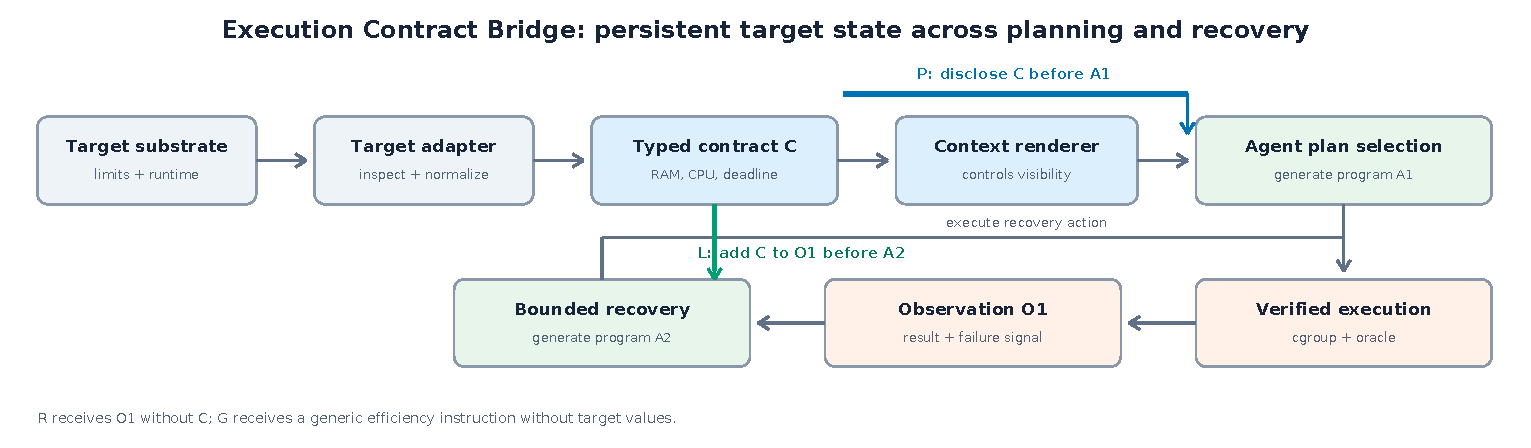
\includegraphics[width=0.98\textwidth]{figures/contract_bridge_architecture}
  \caption{Execution Contract Bridge and bounded agent loop. The same inspected
  target, typed contract, executor, and verifier serve every condition. P exposes
  the contract before the first action; R supplies only the authentic observation
  at recovery; the matched late-disclosure extension L adds the exact contract to
  that same observation before the second action.}
  \Description{A system diagram shows target inspection and contract compilation,
  context rendering, agent plan selection, verified execution, observations, and
  bounded recovery. Blue and green paths mark proactive and late contract disclosure.}
  \label{fig:bridge}
\end{figure*}

\subsection{Information conditions}

All conditions receive the identical task, runtime/package availability, safety
rules, generation configuration, executor, and correctness oracle.
\begin{description}
  \item[P---Proactive contract.] The exact target memory, CPU, and wall-time
  limits are visible before the first implementation is selected.
  \item[R---Reactive discovery.] The initial state contains the task but not the
  target limits. If the first program is unsuitable, its authentic exit status,
  timeout/OOM signals, and captured output are supplied for one recovery attempt.
  \item[G---Generic efficiency.] The initial prompt requests balanced memory and
  time efficiency without target values. An unsuitable execution receives the
  same recovery evidence as R.
\end{description}

P tests whether known target state improves first-pass planning. R measures the
work required to react to the boundary through execution feedback. G separates
specific environment information from a generic request for efficient code.

\subsection{State and timing model}

Let $B=(T,V)$ denote the task plus the runtime/dependency state visible in every
condition, $E$ the target environment, and $C=f(E)=(M,Q,\tau)$ the experimentally
manipulated contract containing memory ceiling $M$, CPU quota $Q$, and deadline
$\tau$. (The bridge schema also carries $V$; this study holds it constant.) An agent
policy $\pi$ selects a program $A$ from its observable state; the executor
$X_E(A)$ returns observation $O$, and an independent verifier defines
\begin{equation}
S(A,E)=\mathbb{1}[\mathrm{correct}(A)\land m(A)\le M\land t(A)\le\tau].
\end{equation}
The primary conditions differ only in the information $I$ supplied to $\pi$,
with $A_k^c\sim\pi(\cdot\mid I_k^c)$ and
\begin{align}
I_1^P&=(B,C), & I_1^R&=B, & I_1^G&=(B,g),\\
I_2^P&=(B,C,A_1^P,O_1^P),\nonumber\\
I_2^R&=(B,A_1^R,O_1^R),\qquad
I_2^G=(B,g,A_1^G,O_1^G),
\end{align}
Here $g$ denotes generic efficiency guidance. In a separately frozen extension,
we hold each failed $(B,A_1^R,O_1^R)$ state fixed and change only contract
visibility at recovery:
\begin{equation}
A_2^L\sim\pi(\cdot\mid B,A_1^R,O_1^R,C).
\end{equation}
This design distinguishes whether exact state is useful, when it is useful, and
whether failure symptoms alone carry equivalent information.

\section{Experimental Design}

\subsection{Tasks and opposed environments}

We use two inspectable code-generation families. The numerical family computes a
pairwise-distance aggregate over deterministic dense arrays. Candidate programs
may materialize a quadratic intermediate or use bounded blocking, precision
retention, symmetry, and buffer reuse. The ETL family computes exact conditional,
weighted aggregations over deterministic CSV data. Candidate programs may use
bounded streaming, chunked data frames, or eager vectorized data frames.

Each family contains two independently generated instances with distinct assets,
hashes, task constants, and correctness oracles. Each instance executes in two
calibrated environments. The memory-tight environment admits the bounded strategy
and rejects the opposed eager reference. The latency-tight environment admits the
faster reference and rejects its slower opposed reference. Before any confirmatory
generation, five repeated executions of every expected reference passed and five
of every opposed reference failed under the frozen envelopes.

\begin{table}[t]
  \caption{Frozen execution contracts. Every environment uses one CPU core.}
  \label{tab:contracts}
  \centering
  \small
  \begin{tabular}{llrr}
    \toprule
    Family & Instance & Memory-tight & Latency-tight \\
    \midrule
    Numerical & Primary & 128 MiB, 8.0 s & 1024 MiB, 3.0 s \\
    Numerical & Secondary & 128 MiB, 8.0 s & 1024 MiB, 3.0 s \\
    ETL & Primary & 128 MiB, 4.0 s & 512 MiB, 1.4 s \\
    ETL & Secondary & 128 MiB, 4.0 s & 512 MiB, 1.7 s \\
    \bottomrule
  \end{tabular}
\end{table}

\subsection{Models and sampling}

The confirmatory matrix uses Google Gemini 3.8 Flash, OpenAI GPT-5.6 Sol, and
Anthropic Claude Sonnet 5 at documented medium thinking/effort settings. Provider
manifests freeze model identifiers, output limits, unsupported sampling controls,
prices, call caps, and cost caps. Each model contributes
$2\times2\times2\times3\times4=96$ independently generated trajectories, for 288
total. Repetition indices are bookkeeping identifiers, not statistical pairs.
Execution order is randomized from a frozen seed.

The development canaries and 24-trajectory Gemini pilot were used only to validate
the pipeline, calibrate task opposition, and freeze the confirmatory design. They
are archived separately and are never pooled with confirmatory evidence.

After completing the primary matrix, we froze a recovery-timing extension over
all 82 archived R first-attempt failures. For each state, L reuses the exact task,
failed program, authentic execution observation, provider configuration, and
second-turn scaffold used by R, then adds the target contract before generating a
fresh recovery action. This produces matched comparisons of symptom-only and
exact-contract recovery without rerunning or resampling the initial failure.

\subsection{Execution and scoring}

Generated programs run non-root on a persistent Debian Linux worker with CPython
3.11.2, NumPy 2.0.2, and Pandas 2.2.3. The executor removes network access, mounts
the task asset read-only, limits process creation, constrains CPU and memory using
cgroup v2, caps captured output, and enforces the task deadline. It records cgroup
\texttt{memory.peak}, \texttt{memory.events}, \texttt{cpu.stat}, pressure-stall
information, exit status, stdout/stderr, program time, and supervisor time. A
positive-control preflight verifies that resource enforcement is active.

Suitability requires an independently verified correct result, no timeout or OOM
kill, and execution within both frozen memory and time bounds. Each trajectory
allows one initial attempt and, only after an unsuitable result, at most one
recovery attempt. Provider errors and malformed responses remain in the attempted
run ledger. Only provider failures before any model response may receive a linked
replacement; a provider interruption between attempts may continue only from the
exact archived repair prompt. Both mechanisms are outcome-neutral and preserve
the original record.

\subsection{Endpoints and analysis}

The co-primary estimands are the equal-stratum-weighted risk differences in
verified first-pass suitability for P$-$R and P$-$G across
model$\times$family$\times$instance$\times$environment strata. We report raw
counts and Wilson intervals. Two-sided $p$-values come from 100,000
within-stratum label permutations (seed 20260924), with Holm correction for the
two primary contrasts. Secondary outcomes include final
suitability within two attempts, calls and tokens per successful trajectory,
failed executions, recovery latency, program time, peak memory, exceedance, and a
strategy taxonomy frozen before confirmatory generation. Continuous contrasts
use 20,000 stratified bootstrap resamples (seed 20260925). Failed executions are
reported by type and never assigned invented resource values.

For the matched recovery extension we report the $2\times2$ transition table and
an exact two-sided McNemar test. We also recompute both primary risk differences
after removing, in turn, each model configuration, task instance, family,
environment type, and full model--family--instance--environment stratum. These
removal analyses test whether the conclusion depends on any single component of
the benchmark matrix.

\begin{figure*}[t]
  \centering
  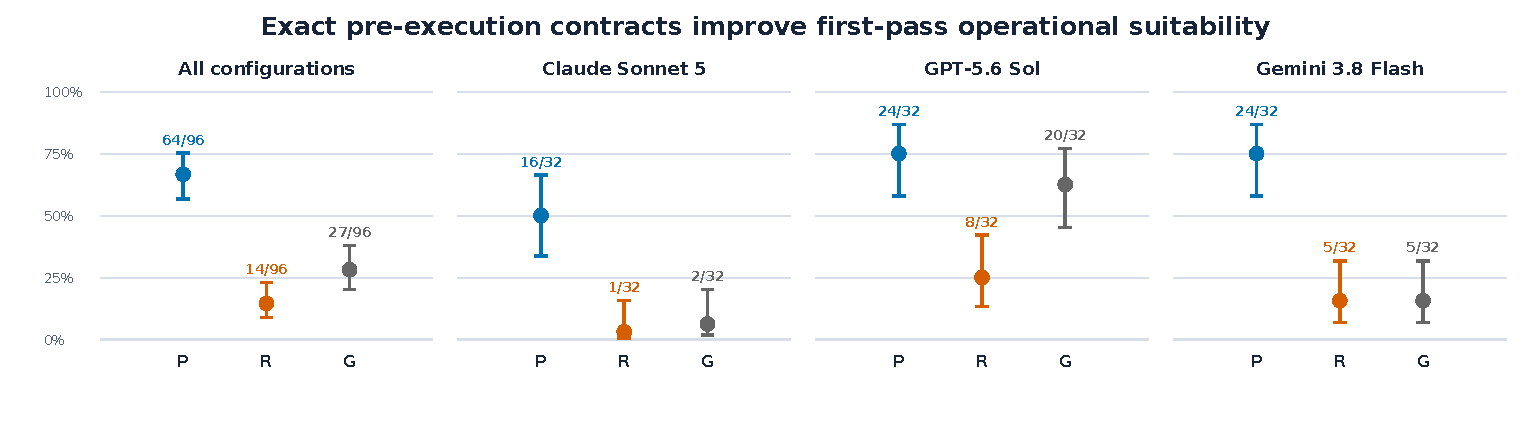
\includegraphics[width=0.98\textwidth]{figures/primary_suitability}
  \caption{First-pass suitability with 95\% Wilson intervals. P outperforms R
  in all three provider-configured models. G approaches P for GPT-5.6 Sol but
  does not reproduce the effect for Claude Sonnet 5 or Gemini 3.8 Flash.}
  \Description{Four panels show proactive, reactive, and generic first-pass
  suitability overall and for each model. Proactive is highest in every panel.}
  \label{fig:primary}
\end{figure*}

\section{Results}

\subsection{First-pass environment suitability}

Proactive contract disclosure produced 64/96 first-pass suitable programs
(66.7\%, Wilson 95\% CI 56.8--75.3\%), compared with 14/96 under reactive
feedback (14.6\%, 8.9--23.0\%) and 27/96 under generic efficiency guidance
(28.1\%, 20.1--37.8\%). The equal-stratum risk difference was +52.1 percentage
points for P$-$R and +38.5 points for P$-$G. Both two-sided randomization tests
returned $p<10^{-5}$ before correction and $p=2.0\times10^{-5}$ after Holm
correction.

The first-pass advantage over R appeared in every model configuration: +46.9
points for Claude Sonnet 5, +50.0 for GPT-5.6 Sol, and +59.4 for Gemini 3.8
Flash. P also exceeded G for every configuration, although the separation was
smaller for GPT-5.6 Sol (+12.5 points) than for Claude (+43.8) or Gemini (+59.4).
Thus generic optimization language can elicit strong behavior in one
configuration, but it does not provide the consistent cross-configuration
reliability of a concrete target contract (Figure~\ref{fig:primary}).

\begin{table}[t]
  \caption{Verified suitability and generation work by information condition.
  Calls and tokens are totals over each fixed 96-trajectory cohort.}
  \label{tab:primary}
  \centering
  \small
  \begin{tabular}{lrrrr}\toprule
  Condition & First pass & Final & Calls & Tokens \\\midrule
  Proactive (P) & 64/96 & 72/96 & 128 & 469k \\
  Reactive (R) & 14/96 & 33/96 & 178 & 596k \\
  Generic (G) & 27/96 & 43/96 & 165 & 671k \\\bottomrule
  \end{tabular}
\end{table}

The first proactive attempt also outperformed the complete two-attempt
alternatives: P produced 64 suitable programs before any recovery, 31 more than
R's final 33 and 21 more than G's final 43. The advantage is therefore visible
against the complete bounded workflows, not only against their initial actions.

\begin{table}[t]
  \caption{First-pass / final suitable trajectories by model ($N=32$ per row).}
  \label{tab:model}
  \centering
  \small
  \begin{tabular}{lrrr}\toprule
  Model & P & R & G \\\midrule
  Claude Sonnet 5 & 16/22 & 1/9 & 2/7 \\
  GPT-5.6 Sol & 24/25 & 8/16 & 20/26 \\
  Gemini 3.8 Flash & 24/25 & 5/8 & 5/10 \\\bottomrule
  \end{tabular}
\end{table}

\subsection{Where contract disclosure changes planning}

The treatment effect follows the environment, rather than a universal ranking of
models or algorithms (Figure~\ref{fig:regime}). In memory-tight ETL, P was
first-pass suitable in 24/24 trajectories, versus 5/24 for R and 13/24 for G. In
memory-tight numerical work, the counts were 22/24 versus 8/24 and 8/24; in
latency-tight numerical work, 17/24 versus 0/24 and 5/24. These three regimes
yield P$-$R advantages of 58.3--79.2 percentage points and P$-$G advantages of
45.8--58.3 points.

Latency-tight ETL is the boundary case: every condition achieved only 1/24
first-pass suitable programs; after one recovery, P and R reached 3/24 and G
reached 5/24. The contract accurately exposed the 1.4/1.7-second deadlines, but
most generated implementations still missed them. Explicit state substantially
improves selection where the models can synthesize a fitting strategy; state
availability alone does not make every calibrated boundary attainable.

\begin{figure}[t]
  \centering
  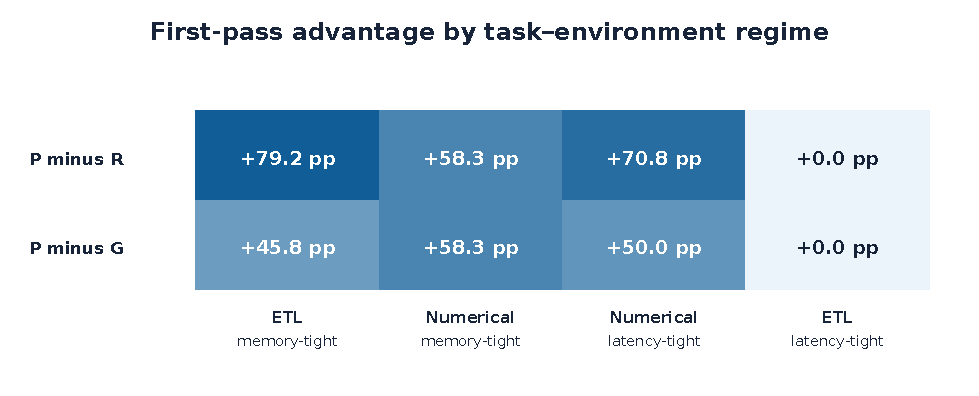
\includegraphics[width=\columnwidth]{figures/effect_by_task_environment}
  \caption{Equal-cell first-pass risk differences by task--environment regime.
  The effect is large in three regimes and absent in latency-tight ETL.}
  \Description{A two-row heat map shows proactive-minus-reactive and
  proactive-minus-generic percentage-point differences across four regimes.}
  \label{fig:regime}
\end{figure}

The generated code reveals structural changes behind these outcomes. In the
numerical family, 42/48 P programs selected blocked matrix computation, and 37/48
explicitly retained \texttt{float32}; the corresponding counts were 29/48 and
1/48 for R, and 42/48 and 13/48 for G. In ETL, 24/48 P programs used explicit
data-frame chunking, compared with 0/48 for R and 21/48 for G. R instead selected
standard-library row streaming in 30/48 cases. The numeric contract therefore
changes both strategy family and lower-level choices such as precision and chunk
geometry; a generic efficiency request sometimes selects the same broad family
without reliably fitting the actual envelope.

\begin{table}[t]
  \caption{First-attempt strategy and suitability. Each cell reports programs
  suitable among programs selecting the strategy. Counts are
  descriptive across the balanced environment mix.}
  \label{tab:strategy}
  \centering
  \scriptsize
  \begin{tabular}{lrrr}\toprule
  Strategy & P & R & G \\\midrule
  Numerical blocked & 33/42 & 8/29 & 13/42 \\
  Numerical eager & 6/6 & 0/16 & 0/5 \\
  ETL data-frame chunked & 11/24 & 0/0 & 8/21 \\
  ETL standard-library stream & 13/15 & 5/30 & 6/14 \\
  ETL eager data frame & 1/9 & 1/18 & 0/13 \\\bottomrule
  \end{tabular}
\end{table}

Table~\ref{tab:strategy} shows why broad algorithm labels alone do not determine
fitness. P and G selected blocked numerical computation equally often, yet
33/42 P programs were suitable versus 13/42 G programs. Conversely, all six P
programs selecting eager numerical computation for the latency-oriented envelope
were suitable. Exact state shapes both the family of strategy and
its target-specific parameterization.

\subsection{Recovery work and resource behavior}

Within the two-attempt limit, final suitability was 72/96 for P, 33/96 for R,
and 43/96 for G. P required 128 calls, versus 178 and 165, and consumed 469k
tokens, versus 596k and 671k (Table~\ref{tab:primary}). Across every issued
execution, P produced 56 unsuitable runs; R produced 145 and G produced 122.
The P cohorts therefore obtained more suitable programs while executing far
fewer failed implementations.

\begin{table}[t]
  \caption{Failure prevention and cohort-level operational yield. OOM and timeout
  counts describe attempt 1; unsuitable executions include both attempts. Yield
  divides total calls or tokens by final suitable trajectories.}
  \label{tab:operations}
  \centering
  \scriptsize
  \begin{tabular}{lrrrrr}\toprule
  & OOM & Timeout & Unsuitable & Calls/success & Tokens/success \\\midrule
  P & 2 & 29 & 56 & 1.78 & 6.5k \\
  R & 24 & 58 & 145 & 5.39 & 18.1k \\
  G & 27 & 42 & 122 & 3.84 & 15.6k \\\bottomrule
  \end{tabular}
\end{table}

Relative to R, proactive disclosure reduced first-attempt OOM kills by 91.7\%
and timeouts by 50.0\%; relative to G, the reductions were 92.6\% and 31.0\%.
Its higher-information prompt did not increase total inference work. P used
24,168 first-attempt input tokens, 8,968 more than R, but only 1,023 more input
tokens across the complete workflow (36,099 versus 35,076). It generated 127,357
fewer output/reasoning tokens and used 21.2\% fewer total tokens than R. Relative
to G, P used 30.1\% fewer total tokens. Up-front state therefore repaid its context
cost through fewer recovery calls and substantially less generated work.

The stratified bootstrap supports the same operational picture. P used 0.52
fewer attempts per trajectory than R, with 95\% interval $[-0.56,-0.48]$, and
0.39 fewer than G, with interval $[-0.44,-0.33]$. It consumed 1,316 fewer
provider tokens per trajectory than R, with interval $[-2{,}027,-618]$, and
2,101 fewer than G, with interval $[-2{,}893,-1{,}314]$. End-to-end trajectory
duration was 5.44 seconds lower than R, with interval $[-9.00,-1.91]$. The
2.51-second difference from G had interval $[-6.72,1.64]$. Final peak memory was lower by 35.1 MiB versus R and
25.4 MiB versus G, with both intervals excluding zero. Final program time was
0.41 seconds lower than R; P and G had comparable final program time. These
secondary measures show that the main gain is not merely eventual correctness:
the contract moves useful work to the first attempt and reduces the recovery
burden.

\subsection{Exact state transforms recovery}

The matched extension establishes that the contract remains valuable after a
failure and that failure symptoms are not an equivalent substitute for target
state. Across the same 82 archived R failures, symptom-only recovery produced
19/82 suitable programs (23.2\%); adding the exact contract to the otherwise
identical recovery state produced 53/82 (64.6\%). The transition table contains
35 improvements, one regression, 18 shared successes, and 28 shared failures
(exact two-sided McNemar $p=1.08\times10^{-9}$; Figure~\ref{fig:recovery}).

\begin{figure}[t]
  \centering
  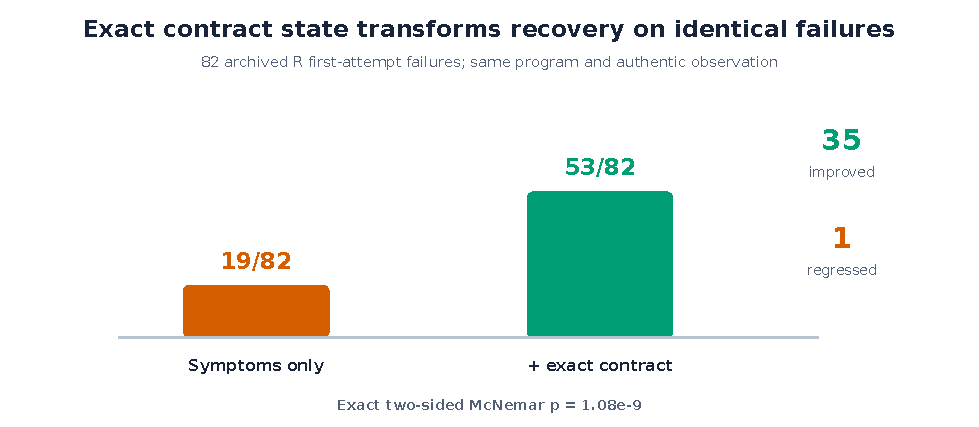
\includegraphics[width=\columnwidth]{figures/matched_recovery}
  \caption{Matched recovery from identical archived first-failure states.
  Exact contract disclosure raises suitable recovery from 19/82 to 53/82.}
  \Description{Two bars compare 19 symptom-only recoveries with 53 exact-contract
  recoveries among 82 matched failures; annotations report 35 improvements and
  one regression.}
  \label{fig:recovery}
\end{figure}

The gain appears for both failure classes: exact-contract recovery succeeded on
18/24 OOM-origin states and 35/58 timeout-origin states, versus 9/24 and 10/58
under symptom-only recovery. No L execution was OOM-killed; its remaining
failures were 27 timeouts and two runtime/correctness errors. By model, recovery
changed from 8/31 to 13/31 for Claude Sonnet 5, 8/24 to 15/24 for GPT-5.6 Sol,
and 3/27 to 25/27 for Gemini 3.8 Flash.

\begin{table}[t]
  \caption{Matched recovery from identical R first-failure states. R receives
  authentic symptoms; L receives the same state plus the exact contract.}
  \label{tab:late}
  \centering
  \small
  \begin{tabular}{lrr}\toprule
  Failure subset & R recovered & L recovered \\\midrule
  Claude Sonnet 5 & 8/31 & 13/31 \\
  GPT-5.6 Sol & 8/24 & 15/24 \\
  Gemini 3.8 Flash & 3/27 & 25/27 \\
  OOM origin & 9/24 & 18/24 \\
  Timeout origin & 10/58 & 35/58 \\
  \textbf{All matched states} & \textbf{19/82} & \textbf{53/82} \\\bottomrule
  \end{tabular}
\end{table}

Viewed as complete two-action workflows, R plus late contract disclosure reaches
67/96 final suitable trajectories, compared with 33/96 for symptom-only R. The
proactive workflow reaches 72/96 while using 128 model calls and 469k tokens;
the late-contract workflow uses 178 calls and 632k tokens because every trajectory
must first attempt to act without the target state. This is 50 fewer calls and
162,901 fewer tokens---a 25.8\% reduction relative to the late workflow's 632,269
total. Proactive and late workflows
are separately sampled at the first action, so this workflow comparison is
descriptive; the 82-state recovery comparison above is fully matched.

The headline result is not carried by a single component of the matrix. After
removing any one model, P$-$R remains +48.4 to +54.7 points and P$-$G remains
+28.1 to +51.6 points. Removing either instance yields +47.9 to +56.2 and +31.2
to +45.8 points, respectively. Both advantages also remain positive after
removing either task family, either environment type, or any one of the 24 full
strata (Table~\ref{tab:removal}). The effect therefore survives every
prespecified structural removal.

\begin{table}[H]
  \caption{Removal robustness of the equal-stratum first-pass suitability
  advantage (percentage points). Each range covers every leave-one-out result;
  positive values favor proactive disclosure.}
  \label{tab:removal}
  \centering
  \small
  \begin{tabular}{lrr}
    \toprule
    Removal & P$-$R & P$-$G \\
    \midrule
    None (full matrix) & +52.1 & +38.5 \\
    Any model & +48.4--+54.7 & +28.1--+51.6 \\
    Either instance & +47.9--+56.2 & +31.2--+45.8 \\
    Either family & +39.6--+64.6 & +22.9--+54.2 \\
    Either environment & +35.4--+68.8 & +25.0--+52.1 \\
    Any full stratum & +50.0--+54.3 & +35.9--+41.3 \\
    \bottomrule
  \end{tabular}
\end{table}

\section{Discussion}

The design tests a concrete architectural proposition: target constraints that
already exist in the execution system should be represented as observable agent
state before implementation selection. P receives that exact state before acting;
R must infer a response from a failed or unsuitable execution, and G begins with
general efficiency intent but no target values. The comparison tests the value of
specific, pre-execution environment information beyond generic optimization
guidance and post-execution failure signals.

The opposed environments also reveal the limit of treating ``efficient'' as a
single objective. A memory-minimizing implementation can miss a latency contract,
while a fast eager implementation can violate a memory ceiling. Substrate-aware
planning therefore concerns suitability for a particular target, not a universal
ranking of algorithms or models.

The distinction between P and G is particularly informative. GPT-5.6 Sol often
translated generic guidance into a suitable implementation, while the other two
configurations did not. Yet the proactive condition remained the only condition
that was consistently strong across providers and opposed envelopes. Execution
contracts replace model-specific interpretations of ``efficient'' with an
explicit target objective, producing substantially more consistent suitability
across providers and opposed execution environments.

The timing experiment sharpens the architecture. Symptom-only feedback raised R
from 14/96 to 33/96, whereas exact state at the same recovery point raised the
workflow to 67/96. The contract should therefore persist across the trajectory:
the harness exposes it before the first action to prevent unsuitable choices and
again alongside authentic observations when recovery is required. This design
combines proactive planning with evidence-grounded repair rather than treating
them as competing paradigms.

\subsection{Threats to validity}

The evaluation covers two code-generation families, three provider-configured
models, this agent loop, and the calibrated environments described above.
Provider outputs are stochastic and model services evolve, so manifests preserve
exact identifiers, settings, timestamps, and raw responses. The deterministic
tasks make operational outcomes auditable but do not represent every software
engineering workload. Strategy labels are secondary behavioral evidence;
execution-derived correctness and resource admission determine suitability.

The target worker is one controlled Linux configuration. This choice holds the
substrate constant while manipulating its observability. Future evaluations can
test portability across accelerators, runtimes, tools, quotas, and dynamically
changing environments using the same adapter/contract boundary.

\subsection{Artifact and reproducibility package}

The anonymous supplement preserves the preregistration, frozen prompts and task
manifests, exact model identifiers and inference settings, all effective and
interrupted trajectory records, generated programs, execution evidence, scoring
and analysis code, machine-readable result tables, and source hashes. It also
contains the 82 matched recovery branches and a manifest linking every packaged
file to its archived source. The complete statistical analysis and all figures
can be regenerated offline without provider calls; fresh execution requires a
Linux host with delegated cgroup v2 controllers. This package makes the reported
agent decisions, failures, recovery transitions, and operational measurements
independently auditable.

\section{Related Work}

ReAct couples reasoning and acting through environment observations
~\cite{yao2023react}. Reflexion and Self-Refine use feedback to revise later
outputs~\cite{shinn2023reflexion,madaan2023selfrefine}. LEVER verifies and reranks
generated programs with execution results~\cite{ni2023lever}. SWE-bench supplies
executable repository tasks~\cite{jimenez2024swebench}, while SWE-agent designs an
agent--computer interface~\cite{yang2024sweagent}. These systems establish the
value of acting on execution observations. Our matched R--L comparison identifies
the additional information value of exposing the exact operating boundary
alongside the same authentic failure observation.

EffiBench and Mercury evaluate the execution efficiency of generated code
~\cite{huang2024effibench,du2024mercury}. A single-task precursor introduced
substrate blindness through prompt-level RAM/time disclosure and local process
measurement~\cite{agrawal2026substrate}. The present study turns that proof of
concept into a reusable agent architecture, enforces contracts on Linux, broadens
the task and environment matrix, and isolates both pre-action and matched
recovery-time disclosure. PeakBench independently demonstrates resource-aware
planning for parallel tool invocation: it separates dependency planning from
physical scheduling and finds that resource disclosure reduces avoidable
overflows~\cite{chen2026peakbench}. The implementation an agent synthesizes and
the tools it schedules are complementary decision boundaries. Together, these
results place operational resources inside the agent decision problem rather
than evaluating them only after a plan is fixed.

Recent contract-centered agent work provides a complementary foundation.
Agent Contracts formalizes multidimensional resource governance and budget
delegation for autonomous agents~\cite{ye2026agentcontracts}. Contract-Grounded
Behavior Tree Synthesis exposes robot capabilities and runtime constraints through
an MCP interface before an agent synthesizes a plan~\cite{salfity2026contractgrounded}.
The Execution Contract Bridge addresses the implementation layer: it derives a
typed contract from a concrete execution target, controls when that state becomes
visible, and measures the resulting programs under the target's enforced physical
resource envelope. The matched recovery experiment further isolates disclosure
timing while preserving the authentic failed action and observation.

Resource-aware scheduling traditionally treats CPU, memory, and deadlines as
system-level constraints. Linux cgroup v2 exposes enforceable resource controls
and accounting~\cite{linuxcgroupv2}. The Execution Contract Bridge projects the
decision-relevant portion of that system state into the agent loop while retaining
kernel evidence as the arbiter of operational suitability.

\section{Conclusion}

Execution constraints are not incidental metadata: they help define which
implementation is suitable. This work turns those constraints into typed,
provenance-bearing agent state and evaluates their proactive use against reactive
feedback and generic efficiency guidance. Across 288 trajectories, proactive
contracts raised first-pass suitability from 14.6\% under reactive feedback and
28.1\% under generic guidance to 66.7\%, while reducing failed executions,
calls, and tokens. The effect reproduced across all three model configurations
and three of four task--environment regimes. Across 82 matched failures, exact
state raised recovery from 19/82 to 53/82, demonstrating that contract visibility
remains decisive after an unsuitable action. Both primary advantages survive
removal of any model, task instance, family, environment type, or individual
stratum. The Execution Contract Bridge provides a concrete foundation for agents
that carry the target operating contract through planning, execution, and recovery.

\balance
\bibliographystyle{ACM-Reference-Format}
\bibliography{references}

\end{document}
